\chapter{Implementacja algorytmu}

Implementacja algorytmu została wykonana w języku C++ z zastosowaniem standardowych bibliotek tego języka. Stworzony program to aplikacja konsolowa bez interfejsu użytkownika. Brak GUI motywowany jest koniecznością automatycznego wykonywania kodu na całej bazie danych obrazów. Dodatkowo aplikacja stanowi jedynie pomocnicze narzędzie do testowania wymyślonego algorytmu. Aplikacja składa się z trzech części modelu odcisku, czyli logicznego zapisu minucji dla każdego palca, silnika kodującego oraz silnika porównującego kody. Aplikacja jest jednowątkowa natomiast wszystkie funkcje napisane są w taki sposób aby w razie konieczności łatwo przerobić kod na wiele wątków. Aplikacja nie operuje na obrazach. Minucje są wydobywane za pomocą programu MINDTCT\footnote{Program MINDTCT jest częścią aplikacji NIST Fingerprint Image Software 2 wydaną przez Image Group of the National Institute of Standards and Technology}. Aplikacja jako wejście przyjmuje pliki .xyt zawierające położenia XY i kąta kolejnych minucji odcisku. Minucje oddzielone są znakiem enter. 
\newpage
\section {Diagram klas}
\begin{figure}[!hb]
    \begin{center}
		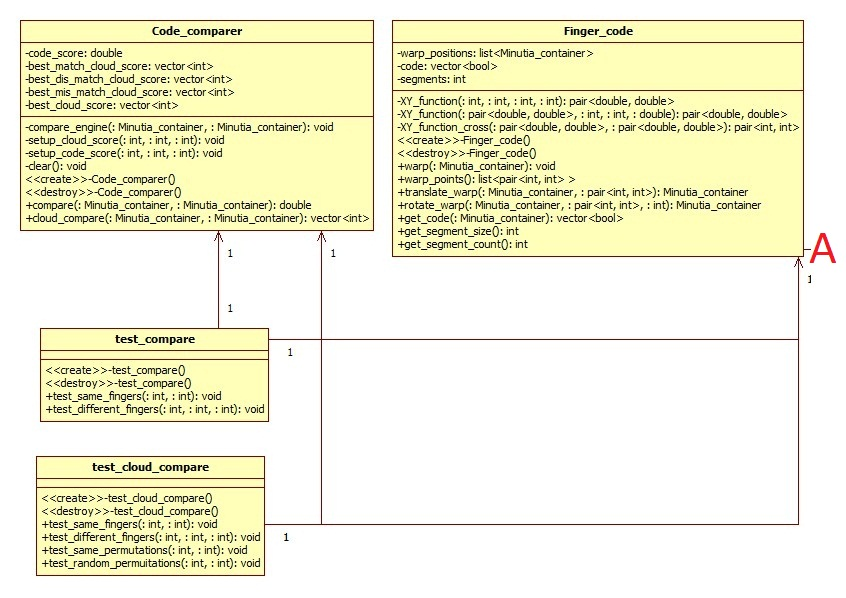
\includegraphics[angle=90,scale=.9]{img/UML_diagram_1.jpg}
		\caption{Diagram klas}
		\label{img:UML}
    \end{center}
\end{figure}
\newpage 
\begin{figure}[!hb]
    \begin{center}
		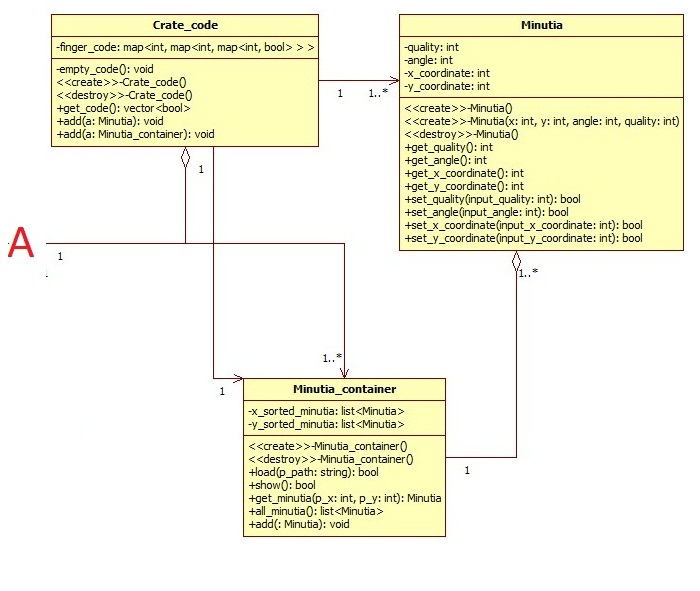
\includegraphics[angle=90,scale=.9]{img/UML_diagram_2.jpg}
		\caption{Diagram klas}
		\label{img:UML}
	\end{center}
\end{figure}

\section {Spis klas}
\begin{enumerate}
	\item Minutia
	\renewcommand*{\labelitemi}{\bullet}
	\begin{itemize}
		\item Klasa odzwierciedlająca fizyczny obiekt minucja. Stworzona do przechowywania podstawowych danych o minucji.
		\begin{itemize}
			\item kąt
			\item jakość
			\item położenie $x$
			\item położenie $y$
		\end{itemize}
		Klasa posiada podstawowe funkcje do zapisu i odczytu przechowywanych wartości.
	\end{itemize}
	\item Minutia\_container
	\renewcommand*{\labelitem}{\bullet}
	\begin{itemize}
		\item Klasa odzwierciedlająca fizyczny odcisk palca. Jest prostym kontenerem przechowującym Obiekty klasy $Minutia$. Jako kontener zastosowano $std::list$. Klasa przechowuje minucje posortowane po 
		współrzędnych, zarówno dla $x$ jak i $y$. 
		\begin{itemize}
			\item lista minucji posortowanych po współrzędnej $x$
			\item lista minucji posortowana po współrzędnej $y$
		\end{itemize}
		Klasa posiada funkcje do wczytywania listy minucji z pliku $.xyt$, Dodawania pojedyńczego obiektu typu $Minutia$, zwracania minucji po współrzędnych, zwracania wszystkich minucji, oraz mechanizm 
		wyświetlający wszystkie minucje na oknie konsoli(używane do debugowania). 
	\end{itemize}


	\item Crate\_code
	\renewcommand*{\labelitem}{\bullet}
	\begin{itemize}
		\item Klasa przechowująca pojedynczą zakodowaną transformacje na obrazie minucji. Jest fizyczną reprezentacją naiwnego kodu odcisku. 
		\begin{itemize}
			\item Naiwny kod
		\end{itemize}
		Klasa pozwala na dodawanie minucji oraz zbioru minucji do zakodowania. Posiada funkcje zwracającą utworzony kod, kod jest tworzony na bieżąco w momencie dodawania minucji.
	\end{itemize}
	\item Finger\_code
	\renewcommand*{\labelitem}{\bullet}
	\begin{itemize}
		\item Klasa przechowująca macierz kodów odcisku. Jest fizyczną reprezentacją całego kodu odcisku. Właściwie w funkcjach tej klasy zakodowany jest cały algorytm tworzący kod odcisku.
		\begin{itemize}
			\item Kod odcisku
			\item Liczba segmentów kodu
			\item Lista punktów transformacji obrazu(reprezentowana jako minucje do których należy przesunąć obraz)
		\end{itemize}
		Klasa posiada funkcje do zwrócenia kodu odcisku, pobrania rozmiaru segmentu kodu, liczby segmentów, oraz funkcje dokonujące transformacji obrazu.
	\end{itemize}
	\item Code\_comparer
	\renewcommand*{\labelitem}{\bullet}
	\begin{itemize}
		\item Klasa obliczająca stopień dopasowania odcisków, jest fizyczną reprezentacja funkcji porównującej kody. W zależności od wywoływanej funkcji zwraca odpowiedni współczynnik dopasowania. Działa w 
		dwóch trybach zwracając liczbę minucji dopasowanych i niedopasowanych, lub oblicza współczynnik dopasowania na podstawie podanych wag. 
		\begin{itemize}
			\item najlepszy współczynnik dopasowania
			\item liczby dopasowań, niedopasowań, maksymalizujące liczbę porównań 1:1
			\item liczby dopasowań, niedopasowań, minimalizujące liczbę porównań 1:0
			\item liczby dopasowań, niedopasowań, minimalizujące liczbę porównań 0:1
			\item najlepszą liczbę dopasowań, niedopasowań, arbitralnie wybrany wskaźnik maksymalizujący liczbę porównań 1:1
		\end{itemize}
		Klasa posiada silnik porównujący podane kody, oraz metody obliczające dopasowanie dla dwóch trybów działania.
	\end{itemize}
	\item Test\_compare
	\renewcommand*{\labelitem}{\bullet}
	\begin{itemize}
		\item Klasa do testowania mechanizmu porównywanie poprzez obliczanie współczynnika porównań.
	\end{itemize}
	\item Test\_cloud\_compare
	\renewcommand*{\labelitem}{\bullet}
	\begin{itemize}
		\item Klasa do testowania mechanizmu porównywanie poprzez obliczanie liczby dopasowań niedopasowań.
	\end{itemize}
	\item Config.h
	\renewcommand*{\labelitem}{\bullet}
	\begin{itemize}
		\item Plik nagłówkowy zawierający elementy konfiguracji programu.
	\end{itemize}
\end{enumerate}



\begin{lstlisting}[language=C++,style=outcode,caption=Przykładowa konfiguracja]
/*
 * Config.h
 *
 *  Created on: 2011-05-07
 *      Author: czareq
 */

#ifndef Config_H_
#define Config_H_

#include <limits.h>

#define ERROR INT_MAX
#define MIN_SCORE INT_MIN
const double PI = 3.14159265358979323851280895940;

/*
 * code parameters
 */
const int X_CODE_RES = 300;
const int Y_CODE_RES = 300;
const int ANGLE_RES = 300;
const int CODE_SEP = 25; 
const int CODE_ANGLE_SEP = 30;

/*
 * warper parameters
 */
const double COVER_STEP = 0.5; 
const int X_STEP = (int) (COVER_STEP * CODE_SEP);
const int Y_STEP = (int) (COVER_STEP * CODE_SEP);
const int ANGLE_STEP = 15;
const int ANGLE_STEP_RANGE = 45;

/*
 * comparer parameters
 */
const int MATCH_POINT = 500;
const int DIS_MATCH_POINT = 500;
const int MIS_MATCH_SCORE = 100;
#endif /* Config_H_ */
\end{lstlisting}
\section {Przebieg procesu weryfikacji}

\begin{enumerate}
	\item Wyodrębnienie listy minucji minucji
	\renewcommand*{\labelitem}{\bullet}
	\begin{itemize}
		\item MINDTCT ekstrakcaj minucji wzorca i próbki
		\item Zapis do pliku $.xyt$
	\end{itemize}
	\item Tworzenie modeli
	\renewcommand*{\labelitem}{\bullet}
	\begin{itemize}
		\item Wczytanie plików $.xyt$
		\item Utworzenie obiektu $Minutia\_container$ dla wzorca i dla próbki oraz zapisanie w nich obiektów $Minutia$
	\end{itemize}
	\item Tworzenie kodów
	\renewcommand*{\labelitem}{\bullet}
	\begin{itemize}
		\item Utworzenie obiektu $Crate\_code$ dla wzorca
		\item Utworzenie obiektu $Finger\_code$ dla próbki
		\item Zakodowanie próbki
		\begin{itemize}
			\item Utworzenie listy wszystkich translacji
			\item Utworzenie listy obrotów dla każdej translacji
			\item Utworzenie obiektu $Crate\_code$ dla każdej transformacji
			\item Dodanie obiektów $Crate\_code$ do obiektu $Finger_code$
		\end{itemize}
	\end{itemize}
	\item Weryfikacja
	\renewcommand*{\labelitem}{\bullet}
	\begin{itemize}
		\item Utworzenie obiektu $Code_compare$
		\item Pobranie kodu wzorca
		\item Pobranie kodu próbki
		\item Podział kodu próbki na segmenty
		\item Porównanie kodu wzorca z każdym z kodów segmentu
	\end{itemize}
	\item Zwrócenie i zapisanie wyniku
	\renewcommand*{\labelitem}{\bullet}
	\begin{itemize}
		\item Odczytanie najlepszego wyniku porównania
		\item Zapis do pliku
	\end{itemize}
\end{enumerate}